\documentclass[11pt]{article}
\usepackage{geometry}                
\geometry{letterpaper}
\usepackage[]{graphicx}
\usepackage{amssymb}
\usepackage{mhchem}
\usepackage{enumitem}
\usepackage{multicol,caption}

% Highlight text using \hl{text}.
\usepackage{soul}

% Comment packaging:
\usepackage{color}
\usepackage[dvipsnames]{xcolor}
\usepackage[normalem]{ulem}
\newcommand{\nicole}[1]{{\color{Green}#1}}


\newenvironment{Figure}{\par\medskip\noindent\minipage{\linewidth}}{\endminipage\par\medskip}


\begin{document}

\begin{center}
{\LARGE Quantum Cellular Automata for the Analysis of Entanglement Complexity in Quantum Many-Body Systems }
\vspace{2mm}
{\large \\ Patrick Rall - Undergraduate Junior in Physics, Caltech Class of 2016}
{\large \\ Advised by Nicole Yunger Halpern and Ning Bao, John Preskill Theory Group \\  Institute for Quantum Information and Matter, Caltech}


\end{center}

\begin{abstract}
    Quantum information science often benefits from quantum extensions of classical game theory. Cellular automata are one-player games used in classical studies to generate complexity. Quantum cellular automata can be similarly used to study the complexity of quantum many-body systems. Since block cellular automata like Critters are defined by a local unitary operation they can easily be generalized using quantum circuits. A two or three-qubit quantum circuit is extended to a time evolution acting on an entire $N$-qubit grid. Many quantum block cellular automata can be simulated exactly using a matrix product state despite exhibiting exotic entanglement structure, hence providing a testbed for measures of entanglement complexity. In this analysis we investigate graphs formed by measures on two-qubit subsystems including mutual information, negativity and quantum concurrence. Additionally, resulting states are compared to real-world systems in terms of area laws and correlation-length decay. 
\end{abstract}

\begin{multicols}{2}

\section*{Introduction}
The Game of Life is a cellular automaton developed by the British mathematician John Conway. Featuring a 2D grid of cells that can be either `dead' or `alive' and rules governing the evolution of the cells' states, this simple system evolves complex, sometimes chaotic behaviors that model real-life processes. By extending this model to permit quantum superpositions of `dead' and `alive' cells, we can explore statistical physics of quantum many-body systems. The resulting time evolution is not 
\nicole{[I recommend inserting ``necessarily.'' Someone might engineer a QGoL inspired by a real-life Hamiltonian. Such a QGoL would strengthen physicists' justifications for studying QGoLs, so I recommend against ruling out the possibility of such engineering.]}
based on real-life Hamiltonians, but instead is geared to produce states exhibiting particular kinds of entanglement complexity. 

There are several methods \nicole{[In the interest of preciseness, and in the interest of giving your reader a heads-up, I recommend replacing ``several'' with a number or with ``at least [number].'']} 
for quantizing cellular automata, each with advantages and disadvantages. 
One approach studied \sout{by} \nicole{in [Papers aren't things of the sort that can study; humans are. ;) ]} \cite{Bleh} encodes the update rule of Conway's Game of Life \hl{-} 
\nicole{[According to an APS style guide, such a dash between two words should involve three hyphens and no spaces: ``Life---changing.'']}
changing a cell's state based on the number of alive neighbors \hl{-} into 
a Hamiltonian reminiscent of some condensed\nicole{-}matter systems. 
This analogy creates a reversible quantum update rule inspired by an irreversible classical rule, which causes the quantum version to behave very differently from the original. 
\nicole{[ $\leftarrow$ Can break that sentence in two. I appreciate your having kept a lookout for run-on sentences in this report. :) I'm seeing far fewer than in earlier writing. As a result, I can take in your ideas much more easily when reading this report. We tend to be able to swallow small chunks more easily than huge ones. A few opportunities to shorten sentences remain, though. I hope you're not discouraged by my pointing them out. You're relating high-quality material; I want to ensure that readers can digest it as well as possible.]}
\hl{Extrapolating reversible time evolution present in closed quantum systems is also an issue} 
\nicole{[ $\leftarrow$ Sounds a bit awkward, and I'm not sure what the phrase is supposed to mean. Rewording recommended.]}
for elementary cellular automata 
\nicole{[Does your reader know what an elementary cellular automaton is?]}
which are largely irreversible. The only reversible rules consist of trivial behavior, e.g.\nicole{,} flipping a cell's state or shifting the board one bit to the left.  

As Norman Margolus argues in \cite{Margolus}\nicole{,} an irreversible rule can cause the system to evolve from a complex initial configuration to a short-period cycle. If a cellular automaton (CA) 
\nicole{[Great that you introduce acronyms parenthetically, as APS guidelines stipulate that we should. I recommend introducing this acronym after your first use of the term ``cellular automaton,'' in the first line of the introduction, and using ``CA'' thereafter.]}
has a reversible update rule, the only way it can cycle is by reaching its initial state, 
\nicole{[I recommend splitting this sentence in two here.]}
causing the average cycle period to be significantly longer. 
\nicole{[The foregoing sentence suggests that ``CA must return to initial state in order to cycle'' directly implies ``average cycle period is long.'' Does the former directly imply the latter? Or does the former imply the latter when combined with, say, ``CA must explore all of its large state space before returning to its initial state''?]}
Since reversibility appears to have a significant effect on the CA's emergent properties, \hl{building an analogy between reversible and irreversible CAs}
\nicole{[$\leftarrow$ Can we sharpen this phrase, make it make more precise? Do you mean, say, ``constructing a reversible quantum CA from a classical irreversible CA''?]}
may result in the quantum \sout{case} \nicole{CA's [``CA'' is more precise than ``case.'' The possessive ('s) is required because the result is not the quantum CA, but the quantum CA's being incomparable to the classical CA (an explanation appears in Strunk and White's \emph{Elements}).]} \sout{no longer} \nicole{[$\leftarrow$ Can shorten to one syllable $\to$]} being \nicole{in}comparable to the classical \sout{case} \nicole{CA [for preciseness]}.

To avoid this\nicole{,} I shall focus on block cellular automata discussed in \cite{Margolus}, 
\nicole{[Opportunity to split this sentence in two]}
which involve partitioning the board into small pieces of equal size and shape\nicole{, then} \sout{and} applying a reversible transform to these pieces. This process is repeated over several possible partitionings of the board, resulting in non-trivial but reversible evolution. The `Critters' rule is \sout{an example of}  \nicole{[$\leftarrow$ Unnecessary]} a block cellular automaton which is known to replicate many \sout{of the} \nicole{[$\leftarrow$ Unnecessary]} interesting emergent properties of Conway's Game of Life.  \nicole{[Motivation for using Critters \checkmark]}
The classical rule can be generalized to 
\sout{the quantum case} \nicole{a quantum rule, [(1) More precise. (2) Comma needed.]}
as \hl{reversible transforms can be represented via by unitary operators.} 
\nicole{[The foregoing clause suggests that every reversible transformation can be represented by a unitary. But consider a general invertible matrix $M$ whose inverse is $M^{-1}$. In general, $M$ isn't unitary. That is, in general, $M^{-1} \neq M^\dag$.]}
By \hl{extending these operators via quantum gates,}
\nicole{$\leftarrow$ I suspect that readers won't know what you mean.} 
\hl{quantum properties}
\nicole{$\leftarrow$ In the interest of precision and detail, I recommend clarifying what you mean by ``quantum properties.'' Such a clarification would lengthen an already-somewhat-long sentence. So (surprise, surprise!) I recommend chopping up the sentence.}
can be introduced into the CA in a more controlled manner than 
in \hl{the Hamiltonian case} \nicole{[$\leftarrow$ Vague.]} because \hl{reversibility is preserved.} \nicole{$\leftarrow$ More specific: ``mapping the classical block transformation  to a unitary preserves reversibility.''}


\section*{Methods}

\subsection*{Rule formalism}

\nicole{[As soon as we introduce notation (e.g., $U_k$ and $\mathbb{U}_{i}$), we need to specify what the notation denotes. Often, when a ``set-up'' and lots of notation are introduced, one begins with, e.g., ``Consider an $N$-qubit system that begins in the state $| \Psi \rangle$. Let $U_k$ denote a unitary defined on a subsystem of $k$ qubits. I will call such a $U_k$ an \emph{update rule}.
From $U_k$, we can construct a unitary defined on the $N$-qubit system\ldots''
Also, explaining what $i$ indexes would be useful.]}

Block cellular automata \hl{extend a $k$-qubit update rule $U_k$ to an $N$-qubit system}
\nicole{[$\leftarrow$ I had to think for a while to figure out what the foregoing phrase meant.]}
by transforming a state $|\Psi\rangle$ to $\mathbb{U}_{k-1} ... \mathbb{U}_0 | \Psi \rangle $. 
$\mathbb{U}_i$ can be written in terms of $U_k$ and the $j$-qubit identity gate $\mathbb{I}_j$:
$$\mathbb{U}_i = \mathbb{I}_i \otimes U_k \otimes ... \otimes U_k \otimes \mathbb{I}_{N-i-k[(n-i) \text{ mod } k]}. $$
\nicole{[Is the $n$ in the subscript supposed to be $N$?]}

Since there are $[(N-i)$ mod $k]$ instances of the $U_k$ operator, 
any $\mathbb{U}_i$ acts on an $i + k[(N-i) \text{ mod } k] + N-i-k[(N-i) \text{ mod } k \nicole{]} = N$-qubit system, which is the entire state. The full iteration of the cellular automaton is an application of all possible $\mathbb{U}_i$, i.e., all different possible positions of the $U_k$ operator tiled across the board (see Figure~\ref{fig:block}). This definition is the 1D version of 2D block cellular automata like the `Critters' rule.

\begin{Figure}
\centering
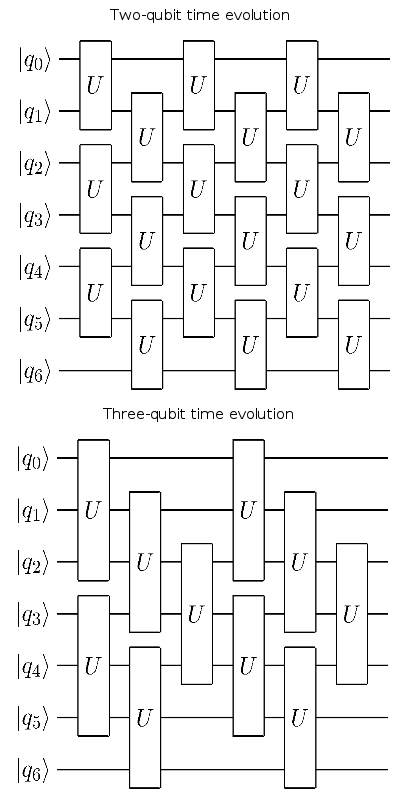
\includegraphics[width=0.8\textwidth]{images_caltech/twoqubittime.png}
\captionof{figure}{\label{fig:block} Quantum circuits showing time evolution of block cellular automata generated by two-qubit or three-qubit gates $U$ for a system with seven sites. Without periodic boundary conditions\nicole{,} some edge qubits must be left unchanged \sout{with} \nicole{at} every step. \nicole{[I recommend mentioning that time progresses from left to right in the diagram.]}}
\end{Figure}



Classical block cellular automata consist of operators $U_k$ defined by a permutation of $k$-bit states. Since a matrix representing a permutation is unitary, such a $U_k$ represents the time evolution of not just a classical system but also a closed quantum system. The quantum update method replicates classical behaviors \hl{in the case of} \nicole{[I recommend replacing this wording, which is a bit vague, with a more precise phrase. For instance: ``The quantum update method replicates classical behaviors if the initial state is neither entangled nor a nontrivial superposition.'']} non-superposed non-entangled initial states\nicole{,} if $U_k$ is entirely a permutation. Such a $U_k$ can be augmented \sout{using} \nicole{with [``Using'' implicitly refers to a person who uses the $U_k$, but such a person is not mentioned in this sentence.]} quantum gates such as the controlled-phase or controlled-Hadamard gates \hl{to introduce quantum behaviors.} \nicole{[A bit vague. Which behaviors are you calling ``quantum''?]} 
While cellular automata consisting purely of quantum gates are also worth studying, the most interesting interactions arise from combinations of classical and quantum update rules. \nicole{[How come?]}

Since there are $2^k$ configurations of $k$-bit states, there are $2^k!$ possible classical permutations. This gives 24 two-bit rules, 40320 three-bit rules and $2.10\cdot10^{13}$ four-bit rules. Due to the size of the classical portion of the rule space, $k\in \{2,3,4\}$ provides a sufficient number of rules for this analysis. 
\nicole{[Good illustration with precise numbers and justification of your choices.]}


\subsection*{Complex networks}

The quantum cellular automata above are simulated using a Matrix Product State (MPS) in canonical form. MPS with open boundary conditions allows constant-time extraction of any single-qubit density matrix and polynomial-time time evolution of the state. These efficiencies are retained\nicole{,} provided the Schmidt-number $\chi$ remains bounded \cite{Orus}, which \hl{is the case for} \nicole{[Again, not my favorite phrase, due to vagueness. :) ]} states with relatively low entanglement complexity. This permits simulation and visualization of cellular automata inside a web-browser with system size $n < 60$
\nicole{[Earlier, you denoted the number of qubits by $N$.]}
\nicole{[Precise numbers \checkmark]}
 and $\chi < 10$. Furthermore, the MPS describes the amount of entanglement between the left half and the right half of \sout{the system} \nicole{a system split} at any \sout{given} point. While this information is useful for understanding the entanglement of simple superpositions like Bell pairs, it is insufficient for more complex behavior. To better characterize states with more complex entanglement, we construct a network 
 \nicole{[Might want to explain what a network is, as many physicists don't use the term much.]}
 whose adjacency\nicole{-}matrix elements $A_{ij}$ are given by some two-point entanglement measure on qubits $i$ and $j$. Measures depending on 2-qubit density matrices $\rho_{ij}$ can be extracted from a MPS in $n^2$ time.

One useful choice \nicole{of\ldots?} is the mutual information $$\mathcal{I}_{ij} = \frac{1}{2}(S_i + S_j - S_{ij}) $$\nicole{,} defined \sout{using} \nicole{in terms of} the von Neumann entropy $S = \text{Tr}(\rho \log \rho) $. 
\nicole{[The foregoing sentence suggests that $\mathcal{I}_{ij}$ is an entanglement measure. I don't believe it is. The study of entanglement measures is a whole sub-field; some QI theorists specialize in entanglement measures. If they read this report, they might object to this characterization of $\mathcal{I}_{ij}$ as an entanglement measure.]}
\nicole{[Ideally, would explain what the subscripted $S$'s denote. In fact, defining  reduced-state density matrices [e.g., 
$\rho_i := {\rm Tr}_{ {\rm all \; qubits \; but} \; i} 
(| {\rm whole \; state} \rangle \langle {\rm whole \; state} |) $
would be helpful and would be consistent with comparable literature.
One natural opportunity to define $\rho_i$ shows up earlier, when you discuss the efficiency with which you can extract a one-qubit density matrix.]}
While containing classical correlations as well as quantum correlations, \sout{it serves as an upper bound for} 
\nicole{$\mathcal{I}_{ij}$ upper-bounds [more precise and more concise]}
\hl{all other  entanglement measures}, 
\nicole{[The foregoing phrase suggests that $\mathcal{I}_{ij}$ is an entanglement measure. Again, I recommend against suggesting so.]}
which is one reason \hl{they} 
\nicole{[They? Do we mean $\mathcal{I}_{ij}$?]}
were chosen for complex network measures in \cite{Carr}. 
An entanglement monotone that \sout{focuses on capturing} \nicole{captures} quantum correlation only is the negativity $$\mathcal{N}_{ij} = \frac{1}{2}(\text{Tr}|\rho_{ij}^{T_i}|-1),$$ based on the positive-partial-transpose criterion for separability. 
\nicole{[Could you please define the superscript $T_i$? Doing so would be consistent with comparable literature.]}
\nicole{[I recommend citing Peres's paper and the Horodecki's paper about the PPT criterion. (The papers appear in the ``References'' section on the relevant Wikipedia page.)]}
Quantum concurrence is another monotone\nicole{,} defined by\sout{:}
$$\mathcal{C}_{ij} = \text{max}(0,\lambda_1 -\lambda_2 - \lambda_3 - \lambda_4)$$\nicole{,}
where $\lambda_i$ are the eigenvalues\nicole{,} in decreasing order\nicole{,} 
of the matrix $\rho_{ij} (\sigma_y \otimes \sigma_y) \rho_{ij}^* (\sigma_y \otimes \sigma_y) $. 
\nicole{[I recommend breaking up the foregoing sentence.]}
\nicole{[I recommend citing a paper or textbook here.]}
\nicole{[Have you defined $\sigma_y$?]}
Each of these measures exhibit\nicole{s} some mathematical properties, e.g.\nicole{,} concurrence exhibits monogamy of entanglement.
\nicole{[Your impulse to specify details by providing an example is good. ``Some mathematical properties'' is rather vague, though. Can we sharpen that phrase? 
Also, I recommend replacing ``exhibit'' with ``describe'' or another verb. ``Exhibit'' doesn't quite suit the context.]}
\hl{Despite this, it is difficult to gain an intuition how these measures compare} 
\nicole{[Could sharpen into a more concise phrase. Example: ``To provide intuitions about how these measures compare, I will present examples\ldots'']}
without studying examples, such as states generated by quantum cellular automata.
\nicole{[Good to motivate your later examples. \checkmark]}

\subsection*{State visualization}



Visualization is the most common method for assessing the output of classical cellular automata, 
\nicole{[I recommend splitting the sentence in two here.]}
so a visualization of quantum many-body systems in the computational basis is essential for a \sout{proper} \nicole{[Unnecessary word]} quantum analogy. Classical cell colors are commonly represented by two colors: black and white. In the quantum case this binary set of possibilities must be extended to represent a single-qubit density matrix. 
\nicole{[Clear explanation of your reasoning \checkmark]}
This is achieved by mapping colors to the surface of the Bloch sphere 
\nicole{[I think you mean that you map the surface of the Bloch sphere to colors (the reverse of the mapping direction you mentioned).]}
as shown in Figure~\ref{fig:colormap}, 
\nicole{[I recommend splitting the sentence in two here.]}
where position is given by $\vec{r}$ defined by\sout{:}
$$\rho = \frac{I + \vec \sigma \cdot \vec{r}}{2}.$$
Here\nicole{,} $\rho$ is the single-qubit reduced density matrix and $\vec \sigma$ is the vector of Pauli matrices.

Since $|\vec r| \leq 1$, $\vec r$ represents a position on or inside the Bloch sphere. States on the surface of the sphere are pure states\nicole{,} while states inside the sphere are mixed states. To achieve a complete representation of $\rho$ in a cell on a grid, 
cell color is taken from the direction of $\vec r$ and border thickness is given by $1- |\vec r|$. When $\vec r = \vec 0$\nicole{,} the qubit is in a maximally mixed state and receives a \hl{special representation}. \nicole{[A bit vague. Phrases with this sort of vagueness seem to be a pet peeve of John's, so I recommend being more specific. :) ]} Some examples are given in Figure~\ref{fig:colorexamples}.



\section*{Discussion}
%\vspace{-1.2cm}
Some particularly interesting quantum circuits are shown in Figure~\ref{fig:circuits}. These circuits generate time evolutions exhibiting many of the properties discussed below. 
\hl{They will be referred to using the labels in the figure.} 
\nicole{[I appreciate your detailed instructions. :) This final instruction, though, seems unnecessary.]}

\hspace{1cm}\\
\hspace{1cm}\\
\hspace{1cm}\\



\begin{Figure}
\centering
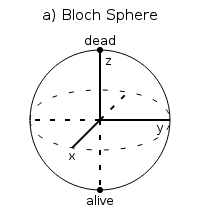
\includegraphics[height=0.4\textwidth]{images_caltech/bloch.png}
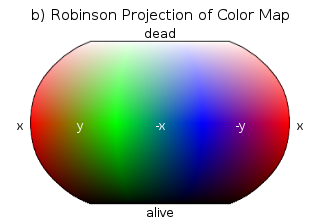
\includegraphics[height=0.4\textwidth]{images_caltech/colormap.png}
\captionof{figure}{\label{fig:colormap} Robinson projection of a Bloch sphere representing the assignment of each qubit state to a color. 
Phase is determined by a cycle over the colors red\nicole{,} green\nicole{,} and blue,
\nicole{[I recommend splitting the sentence in two here.]} 
and \hl{magnitude of components in $|$alive$\rangle$ and $|\text{dead}\rangle$} 
\nicole{[Slight misuse of terminology; rephrasing needed.]}
is determined by overall brightness.}
\end{Figure}
\begin{Figure}
\centering
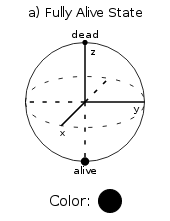
\includegraphics[height=0.4\textwidth]{images_caltech/colorexamples/a.png}
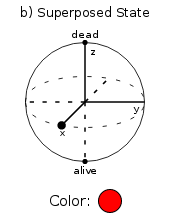
\includegraphics[height=0.4\textwidth]{images_caltech/colorexamples/b.png}
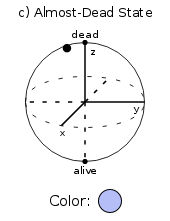
\includegraphics[height=0.4\textwidth]{images_caltech/colorexamples/c.png}
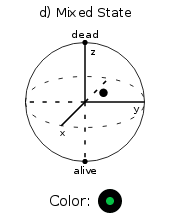
\includegraphics[height=0.4\textwidth]{images_caltech/colorexamples/d.png}
 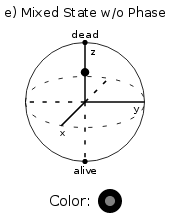
\includegraphics[height=0.4\textwidth]{images_caltech/colorexamples/e.png}
 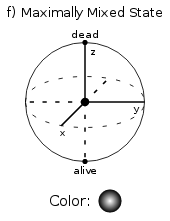
\includegraphics[height=0.4\textwidth]{images_caltech/colorexamples/f.png}
\captionof{figure}{\label{fig:colorexamples} 
\nicole{[Very small suggestion: Figure 3b is labeled ``Superposed State.'' I recommend ``Superposition State.'']
[Good choices of examples. \checkmark]
[I recommend replacing the ``w/o'' in  the label for Fig. 3e with ``without.'' Abbreviations like that are informal don't really belong in formal write-ups.]}
Some examples of single-qubit density matrices\nicole{,} showing \hl{their} \hl{representations} as \hl{a point} inside the Bloch sphere and the color of the corresponding \hl{cell}. \nicole{[Two of the foregoing four highlighted phrases are plural; two are singular. Could we choose either the plural or the singular and use the choice consistently?]}
Direction of the Bloch vector $\vec r$ gives the color, and the degree of \sout{mixing} \nicole{mixedness} $1 - |\vec r|$ gives the border thickness.}
\end{Figure}

\hspace{1cm}\\
\hspace{1cm}\\
\hspace{1cm}\\


\begin{Figure}
\centering

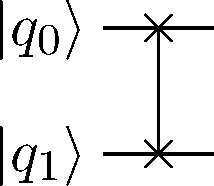
\includegraphics[height=0.15\textwidth]{images_caltech/circuits/U2.png}
\hspace{4mm}
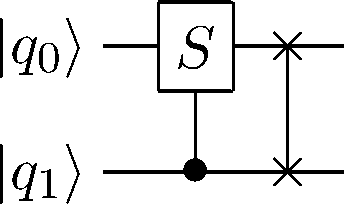
\includegraphics[height=0.15\textwidth]{images_caltech/circuits/U2-S.png}
\hspace{4mm}
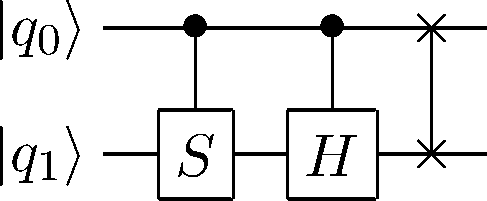
\includegraphics[height=0.15\textwidth]{images_caltech/circuits/trails.png}

\textsc{swap}\hspace{1cm}
\textsc{swap-S}\hspace{1.5cm}
\textsc{swap-HS}
\vspace{5mm}

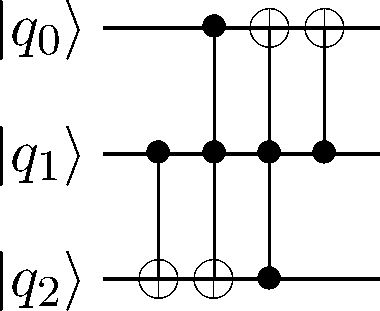
\includegraphics[height=0.3\textwidth]{images_caltech/circuits/U3-2.png}
\hspace{4mm}
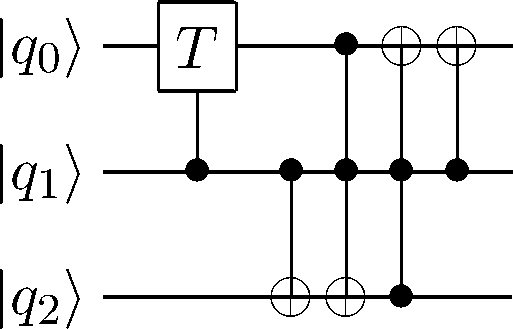
\includegraphics[height=0.3\textwidth]{images_caltech/circuits/U3-2-T.png}

\textsc{twist}\hspace{2cm}
\textsc{twist-T}
\vspace{5mm}

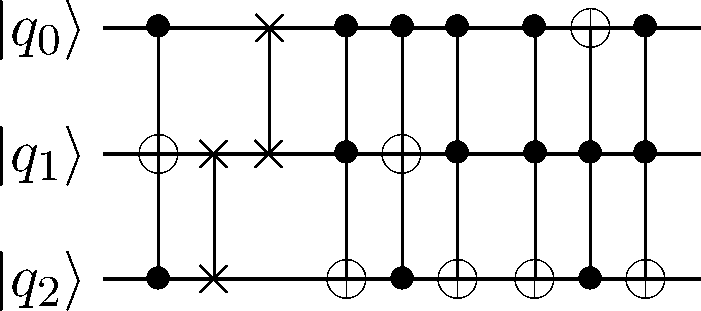
\includegraphics[height=0.3\textwidth]{images_caltech/circuits/U3.png}

\textsc{permute}

\captionof{figure}{\label{fig:circuits} Some examples of quantum circuits generating interesting time evolution when applied as a block cellular automaton. \textsc{swap, twist} and \textsc{permute} are \sout{entirely} \nicole{[Unnecessary word]} classical, so some quantum \sout{modifiers} \nicole{variations} are provided\sout{ as well}.  
\nicole{[What makes the quantum variations quantum? Have you ever explained to the reader? You've explained (very usefully) that permutations are classical. But have you explained what makes a not-just-a-permutation nonclassical?]}}

\end{Figure}



\subsection*{Quantum Gliders}

A useful test for whether quantum block cellular automata yield complex behavior is to see if emergent properties that make Conway's Game of Life interesting can be replicated. The primary \hl{example are} \nicole{[Singular/plural mismatch]} `gliders': if a neighborhood of width $m$ at position $i$ is in configuration $C_{m,i,0}$, a glider represents a structure that undergoes transitions $C_{m,i,0} \to C_{m,i,1} \to C_{m,i,2} \to ... \to C_{m,i+s, 0}$. A glider is a set of configurations that form a cycle\sout{ under a given update rule}, where the configurations move by some offset $s$ with every cycle. These gliders can collide with static structures or other gliders, \sout{which can cause} \nicole{transforming} gliders \nicole{in}to \sout{transform into} other gliders. \nicole{[More concise]}
\nicole{[You provide a mathematical description of a glider and a word-only explanation of a glider. I like both explanations and believe that both, together, provide a well-rounded view of gliders. I recommend putting the word-only explanation first. I found myself scratching my head over the mathematical notation, continuing to the prose explanation, and then understanding the notation. Putting the prose explanation first would enable physicists to visualize a sketch of what you mean. Once they reach the mathematical explanation, they'll be able to grasp your notation.]}

\begin{Figure}
\centering
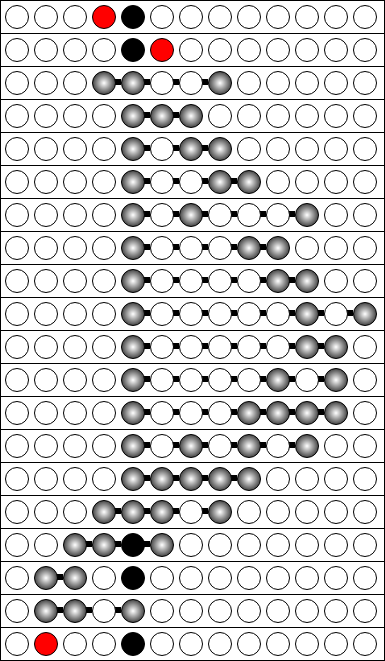
\includegraphics[width=0.9\textwidth]{images_caltech/glider.png}
\captionof{figure}{\label{fig:glider} Time evolution of \textsc{permute}\nicole{,} showing a quantum glider. Time flows from top to bottom. \nicole{\checkmark} Black lines connecting qubits show the von Neumann entropy between the left half and right half of the system. 
\nicole{[Slight rewording recommended:
There can be entanglement between the halves of the system. 
The entropy quantifies the entanglement.
But people tend not to say that ``there is entropy between the halves of a system.'']}
The initial \hl{product state  is of the form $(|C_{i,0}\rangle + |C'_{i}\rangle)/\sqrt{2} $}
\nicole{[I'm afraid I don't understand. How is this a product state?]}
 where $C_{i,0}$ is a glider and $C'_i$ is not. We see $C_{i,0}$ propagates to the right, bounces off the right edge, and then propagates left\nicole{ward}. $C'_i$ is left behind and remains at a constant position.  }
\end{Figure}


Many rules of the form described above \sout{exhibit} \nicole{generate} these structures. In the simplest case, \textsc{swap} yields gliders that consist of single `alive' excitations that move left\nicole{ward} or right\nicole{ward,} given the parity of 
\hl{their position} \nicole{[Single/plural mismatch]} \nicole{initial} $i$. The gate \textsc{permute} exhibits a right-moving glider that conserves \nicole{the} number of \sout{a}live qubits, and a left\nicole{-}moving glider that cycles between three and four \sout{a}live qubits.





These gliders can have quantum properties: if a neighborhood is initialized to a state $(|C_{i,0}\rangle + |C'_{i}\rangle)/\sqrt{2}$\nicole{,} where $C_{i,0}$ is a glider\sout{-}configuration and $C'_i$ is not, half the structure will propagate and the other half will remain stationary. 
\nicole{[Here's a good example of an explanation of what a ``quantum property'' is. \checkmark]}
With most rules, including \textsc{permute}, these structures \sout{will be} \nicole{are} entangled with each other. An example of such a quantum glider is shown in Figure~\ref{fig:glider}.



If an initial state $(|C_{i,0}\rangle + |C_{i,1}\rangle))/\sqrt{2} $ 
\nicole{[Excess of parentheses]}
is prepared, where both configurations are members of the same glider, a structure is formed that is simultaneously in two positions \nicole{steps? [``Positions'' might suggest ``positions on the board,'' i.e., ``cells.'']} of a glider cycle. \textsc{twist} features such a glider that cycles between product states and entangled states\sout{ as it propagates}. \nicole{[Unnecessary words]} Gliders can become entangled with each other after a collision, 
\nicole{[I recommend splitting the sentence here.]}
like with \textsc{swap-S}\nicole{,} where one-qubit \hl{superposed excitations} 
\nicole{[I wasn't sure what that phrase meant.]}
undergo a conditional phase rotation \sout{with} \nicole{during} every collision.



Rules that consist entirely of classical permutations tend to only produce entanglement \sout{complexity} with these quantum gliders, particularly if the bulk of qubits in the $|$dead$\rangle$ state is not a member of any glider cycle.
\nicole{[The foregoing sentence confused me.]}
However, \hl{rules with quantum extensions}\nicole{,} such as controlled-Hadamard\nicole{,} fill the \sout{entire} board with intricate patterns. 
\nicole{[If I didn't know already what you meant, I'd guess that you meant (1) each such rule (which I'll call $R$) corresponds to a rule $R'$; (2) $R'$ is a quantum extension of $R$; and (3) $R'$ fills the board with patterns. But you mean that $R$ is a quantum rule that fills the board with extensions.]}
The entanglement behaviors of large-scale patterns are difficult to characterize by mere inspection, \sout{as was possible with quantum gliders.}
\nicole{unlike quantum gliders' entanglement behaviors}. \nicole{[Clearer, more precise]}

\nicole{[Good segue into the next section. \checkmark]}




\subsection*{Entanglement Structure}

When entanglement structure is \sout{relatively} \nicole{[Unnecessary]} simple, as in Figure~\ref{fig:glider}, \sout{then} \nicole{[Unnecessary]} the entanglement between the \nicole{system's} left and right \nicole{halves,} \sout{half of the system} along with 
\sout{the reduced density matrices of each qubit,} 
\nicole{each qubit's reduced density matrix [More concise; singular/plural mismatch removed; comma needed]}
is often sufficient \sout{information} \nicole{[Unnecessary]} \sout{to understand} \nicole{for understanding [grammar issue]} \hl{what is going on} \nicole{[Informal diction. I don't want for your report to sound distractingly formal, but I recommend using a slightly higher level of prose.]}. For states with more intricate entanglement structure\nicole{,} \hl{this is no longer possible,} \nicole{[Vague]} for instance\nicole{,} in the state shown in Figure~\ref{fig:entangle}. Complex networks are a more sophisticated tool \sout{to query} \nicole{for querying [Grammar issue. Also, I recommend finding a  verb that would suit the context better than ``query'' does.]} the entanglement structure. 

\begin{Figure}
\centering
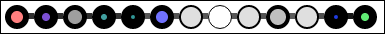
\includegraphics[width=0.95\textwidth]{images_caltech/moreentangled.png}
\captionof{figure}{\label{fig:entangle} A state of entangled qubits generated by \textsc{twist-T}. Individual qubit states are easily determined by their corresponding cells. \hl{Entanglement in this state appears homogeneous in this representation, but upon further analysis with networks of entanglement measures one can see it has a more interesting structure.} 
\nicole{[Great example with which to illustrate your point.] 
[I'm afraid that this final sentence is overloaded with words. Example suggested replacement: ``The entanglement appears homogeneous. Network analysis, though, reveals the entanglement's structure.''] 
[You might want to remind the reader (who's unfamiliar with your diagrams) that the entanglement appears homogeneous because all the links look about equally thick.]}}
\end{Figure} 


\begin{Figure}
\centering
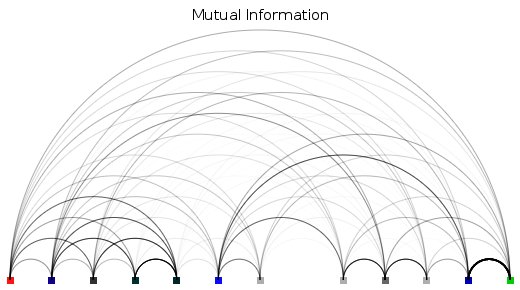
\includegraphics[width=0.9\textwidth]{images_caltech/mutinfonet.png}
\captionof{figure}{\label{fig:mutinfo} Depiction of a mutual\nicole{-}information network of the state shown in Figure \ref{fig:entangle}, \nicole{[I recommend splitting the sentence here.]} where thicker lines mean larger mutual information. This representation shows which qubit is \hl{entangled} \nicole{[But the mutual information doesn't tell us clearly about entanglement. The MI tells us about correlations without specifying which correlations it's telling us about.]} with which other qubit \sout{much} \nicole{[Unnecessary]} \hl{more clearly}. \nicole{[I recommend moving this modifier to just after ``This representation shows.'' Located where it is now, ``more clearly'' seems to describe the entanglement, rather than the diagram.]}
\nicole{[I like how you reveal different facets of the same state in this series of figures.]
[Readers might not realize that each square represents a qubit that's represented, in Fig. 6, by a circle.]}}
\end{Figure}


Figure~\ref{fig:mutinfo} is a representation of a mutual\nicole{-}information network inspired by \cite{Carr}. Details about \sout{the structure of} the entanglement that were invisible in Figure~\ref{fig:entangle} are now visible. While \sout{in Figure~\ref{fig:entangle}} the entanglement appeared homogeneous \nicole{in Figure~\ref{fig:entangle}, [Moved the phrase so that one comma, instead of two, would be needed]} we \sout{can} now observe that \hl{this is not the case}. 
\nicole{[Again, not my favorite phrase! Can pretty much always be replaced with a more precise phrase. Example: ``the entanglement varies from link to link between sites.'']}
Both short-range entanglement and long-range entanglement are present in this state. 
\nicole{[This paragraph suggests that the correlations illustrated by the mutual-information network consist of just entanglement. We know that the correlations consist of entanglement and classical correlations. I know that you, being a conscientious scientist, don't want to mislead your reader. This paragraph, though, runs the risk of overstating entanglement's role. Since entanglement is a hot commodity, readers who don't know you, but who know that the MI doesn't encode just entanglement, might suspect you of hyping your material and might mistrust you in the future. Let's make sure that no one does!]}
We can even make some inferences about the state's history. Since there exists entanglement between opposite ends of the system, but less entanglement with the edges and the center, we can guess that at some point a quantum glider propagated from one side to the other.
\nicole{[Interesting! Is this inference correct? I'm guessing you know, since you generated the state and can check the preceding states in the CA's history.]}

Quantum cell colors \sout{entail a full characterization of} 
\nicole{fully characterize [More concise]}
degrees of freedom local to each qubit. 
A full characterization of entanglement \sout{degrees of freedom} is more difficult to achieve, even with entanglement networks. 
From examples like the GHZ state\nicole{,} 
\nicole{[The GHZ state is a good choice of example. Could you remind readers of the GHZ state's form?]}
we know that \sout{there can exist} \nicole{some} three-qubit entanglement \sout{that} is \hl{invisible from two-qubit subsystems}. 
\nicole{[``Some entanglement is invisible from two-qubit subsystems'' isn't grammatically correct.]}
\sout{This implies that entanglement measures on pairs of qubits could never achieve a full characterization.} 
\nicole{[I recommend replacing this sentence with a more concise, more precise one. Example:
``Hence measures defined on pairs of qubits cannot fully characterize entanglement.'']}
Partial descriptions \sout{are still} \nicole{remain [More concise]} useful, however, as complex network measures were shown to be indicators of phase transitions in \cite{Carr}. 
\nicole{[Good justification for your choices. \checkmark Justifications perhaps more directly relevant to your work include how providing multiple perspectives on entanglement, using different measures, offer a well-rounded picture of the whole.]}


Another difficulty is \sout{that it is difficult to separate} \nicole{separating [More concise]} classical correlation from quantum correlation\nicole{,} given a two-qubit mixed state. 
\hl{Different entanglement measures approach this problem differently, hence yielding varying `perspectives' of entanglement.} 
\nicole{[Wordy and repetitive.]}
Mutual information \sout{is guaranteed to capture} \nicole{captures [More concise]} all quantum correlations, but captures some classical correlations as well.
Negativity, an entanglement monotone, 
\nicole{[Is negativity technically a monotone? 
A function $f$ is an entanglement monotone if $f(\rho)$ decreases monotonically as $\rho$ transforms under any LOCC operation (local operations and classical communication). 
I'm not certain if the negativity satisfies that definition. If it does, could you please cite a paper or textbook that says it does?]}
\hl{is only nonzero if} the two-qubit subsystem is inseparable.
\nicole{[Mathematically correct statements about negativity are delicate; I recommend rewording the foregoing phrase carefully. 
Even the location of the word ``only'' requires precision!
Do you mean that the negativity of a two-qubit system is negative only if the system is inseparable? If and only if?]}
Figure~\ref{fig:negativ} shows that \hl{this restriction} \nicole{[Not sure what you meant by that]} involves losing a lot of information about the entanglement structure. When two-qubit \sout{subsystems} \nicole{reduced states} are extracted from a \nicole{whole-system} state \sout{with} \nicole{that contains} multi-qubit entanglement, some quantum correlations are only visible via residual classical correlations. This shows why mutual information gives a \sout{much} \nicole{[Unnecessary]} richer characterization.
\nicole{[``Characterizes'' is a stronger, more concise verbal phrase than ``gives a characterization.'' I recommend using stronger, rather than weaker, verbal phrases.]}


\begin{Figure}
\centering
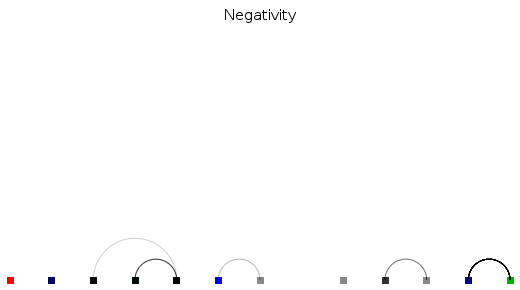
\includegraphics[width=0.9\textwidth]{images_caltech/negativnet.png}
\captionof{figure}{\label{fig:negativ} Depiction of a negativity network for the state shown in Figure \ref{fig:entangle}. \sout{Note that d} \nicole{D}espite the many correlations in Figure \ref{fig:mutinfo}, there appears to be little two-qubit entanglement.  }
\end{Figure}

\begin{Figure}
\centering
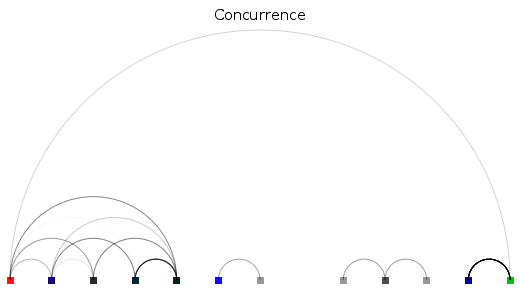
\includegraphics[width=0.9\textwidth]{images_caltech/concurrnet.png}
\captionof{figure}{\label{fig:concurr} Depiction of a concurrence network for the state shown in Figure \ref{fig:entangle}. \hl{This entanglement monotone} 
\nicole{[Is concurrence technically an entanglement monotone?]}
captures more two-qubit entanglement than negativity.  }
\end{Figure}


Other entanglement monotones\nicole{,} like quantum concurrence\nicole{,} exhibit a similar issue: by \hl{restricting to} quantum correlations 
\nicole{[By restricting what to quantum correlations?]}
of two-qubit subsystems we fail to see \hl{other kinds of entanglement.}
\nicole{[What do you mean by ``other kinds of entanglement''? Entanglement between numbers $n > 2$ of bodies? I recommend replacing the highlighted phrase with a more precise description.]}
\nicole{[Is concurrence technically an entanglement monotone (see earlier comment about negativity)? If so, then, when introducing the concurrence, could you please identify the reference that says that the concurrence is a monotone?]}
Comparing Figures~\ref{fig:negativ}~and~\ref{fig:concurr}\nicole{,} we see \nicole{that} concurrence captures more two-qubit entanglement than negativity. Structures that were visible in the mutual\nicole{-}information network in Figure~\ref{fig:mutinfo} are reproduced \nicole{in Fig. 9 only?}, such as the group of five entangled bits on the left and the long\nicole{-}range entanglement between qubits on opposite ends of the board.

\sout{From purely the definitions of monotones like negativity and concurrence, it is difficult to gain intuition on their relative properties.}
\nicole{[I recommend tightening this sentence into a more compact, more grammatically correct one. Example: ``Gaining intuitions about the relationships between the correlation measures is difficult, given just the measures' definitions.'']}
By applying them \nicole{[What do we mean by ``them''? The measures?]} to states generated by quantum cellular automata we can learn more about their characterization of different types of entanglement. This would make their application to real-world many-body systems more practical.
\nicole{[(1) Good to point out how your examples and QCAs can be applied/of use. (2) I recommend trimming unnecessary words from, and sharpening, this paragraph. (3) he paragraph's final sentence suggests that QCAs aren't practical. I recommend focusing instead on QCAs' potential as a testbed.]}

\subsection*{Area Law Analysis and\\ Correlation-Length Decay}

\hl{Quantum cellular automata are not real-world systems, so it is interesting to study how they deviate from reality via analysis tools used to understand condensed-matter systems.}
\nicole{[Good to offer a preview of your main idea in a topic sentence. I recommend tightening the sentence, trimming excess words, and perhaps splitting the sentence in two.]}
Consider the time evolution of \nicole{the} \textsc{swap-HS} cellular automaton \hl{-} 
\nicole{[Form the dash from three hyphens and no spaces.]}
a combination of a classical rule generating moving particles and the controlled-Hadamard gate. 
\nicole{[Does the ``S'' not denote a phase gate?]}
In Figure~\ref{fig:colorful}\nicole{,} \sout{we observe that} a single particle leaves behind a trail of \sout{new} excitations. As the trail bounces across the board\nicole{,} \sout{the states of} the qubits \sout{in the board slowly} homogenize. One could compare this \nicole{behavior} to \nicole{the} dropping \nicole{of} a stone into a puddle: over time\nicole{,} the \sout{single} local excitation will cause the entire board to exhibit excitations that look locally similar.

Many real physical \sout{systems} \nicole{states} obey an area law: the entanglement of a subsystem with its surroundings is proportional to the area of its boundary. 
\nicole{[Citation recommended.]}
This is usually true for states where entanglement is short-range. \nicole{[Citation needed.]} Contiguous subsystems in a one dimensional \sout{state} \nicole{system} have a constant boundary size, so states with an area law would exhibit \sout{subrange} \nicole{[What does ``subrange'' mean?]} entanglement constant in subrange length. \hl{Considering the final state of Figure}~\ref{fig:colorful}, \hl{a plot} of these quantities in Figure~\ref{fig:arealaw} shows that \hl{this is indeed the case.} 
\nicole{[Dangling modifier: ``Considering'' modifies ``a plot.'' But plots aren't things of the sort that can consider. :) A simpler example of a dangling modifier is ``Brewing tea, the phone startled me.'' According to this dangling modifier, the phone was brewing tea! Do you see what I mean and why dangling modifiers need to be avoided?]
[``This is indeed the case'' remains vague\ldots :) ]}
This is on the one hand unsurprising\nicole{,} given the analogy to ripples in a puddle \sout{given above}. On the other hand, the final state in Figure~\ref{fig:colorful} is not fully homogenized, so it is perhaps more surprising that an area law is present so early in the evolution of this system. 
\nicole{[Why is an early-time appearance of an area law surprising? I don't quite see how the surprisingness follows from the information you've provided.]}
This could be a consequence of the small system size.
\nicole{[Great observation and analysis/hypothesis in this last sentence.]}




\begin{Figure}
\centering
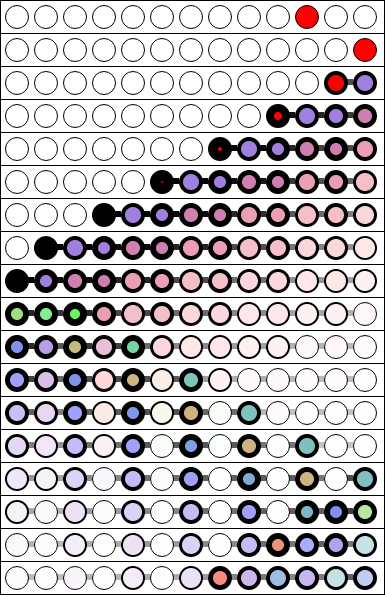
\includegraphics[width=\textwidth]{images_caltech/colorful.png}
\captionof{figure}{\label{fig:colorful} Time evolution of \textsc{swap-HS} starting from a single excitation. 
\nicole{[Might want to mention that time progresses from top to bottom.]}
The cellular automaton is a combination of classical permutations\nicole{, which cause} \sout{causing} particles to move around the board, and the controlled-Hadamard gate\nicole{,} which generates new excitations. \nicole{[Does the S not denote a phase gate?]}}
\end{Figure}

\begin{Figure}
\centering
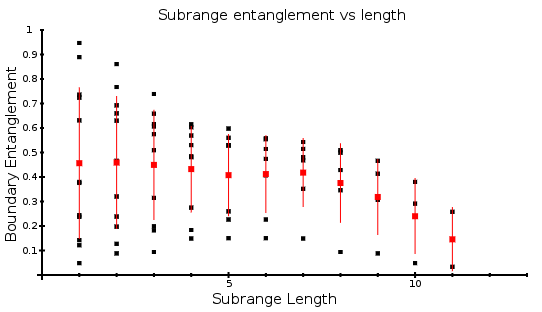
\includegraphics[width=\textwidth]{images_caltech/arealaw.png}
\captionof{figure}{\label{fig:arealaw} Area\nicole{-}law analysis of the final state shown in Figure~\ref{fig:colorful}: \hl{the entanglement of a subrange of qubits with the rest of the system is plotted} against the length of the subrange. 
\nicole{[We can't plot the entanglement directly. Do you mean ``the entanglement entropy''? If so, I recommend changing the caption, the figure's y-axis, and the title atop the figure.]}
Neglecting large subranges ($|i-j| > N/2$)\nicole{,} we observe that subrange entanglement \sout{is constant in} \nicole{is a constant function of [More precise]} subrange length.  }
\end{Figure}


%Measurable

Correlators such as $\langle Z_i Z_j \rangle$ 
\nicole{[Have you defined $Z_i$? Didn't you denote the Pauli matrices by $\sigma_i$ earlier?]}
are commonly used in condensed\nicole{-}matter physics because they \sout{are a quantity that} can be measured in experiments. The \sout{behavior} \nicole{variation} of these correlators \sout{with respect to} \nicole{with} the distance between qubits $i$ and $j$ can \sout{be indicative of} \nicole{signal [More concise]} phase transitions. \sout{Particularly,} equilibrium systems usually exhibit exponential decay of correlation unless the system is close to a phase transition\nicole{,} in which case polynomial decay is observed. 
\nicole{[An arbitrary phase transition? Or only a critical point? I'd recommend (ideally) finding a precise statement in a condensed-matter textbook (e.g., Cardy's, Kardar's second volume) and citing the book here.]}
Figure~\ref{fig:corrdecay} shows the relation between  $\langle Z_i Z_j \rangle$ and $|i - j|$ for the final state in Figure~\ref{fig:colorful}. Rather than \sout{exhibiting a decay} \nicole{decaying [More concise]}, \nicole{the} correlation remains constant as a function of distance. 

While this \nicole{constancy? [What does ``this'' refer to?]} could \sout{be a consequence of} \nicole{result from [More concise]} the final state of Figure~\ref{fig:colorful} not being in equilibrium, 
\nicole{[I recommend splitting the sentence here.]}
simulating the evolution further shows that the lack of correlation decay remains even once the system is fully homogenized. The fact that the system already exhibits an area law \hl{at this time} \nicole{[Which time?]} also suggests equilibrium features could be present. This illustrates that expectations \sout{that are} commonly satisfied by real-world systems can be violated with quantum cellular automata. 
\nicole{[Switching from the passive to the active tense would strengthen the sentence: ``QCAs can violate expectations commonly satisfied\ldots]}
Special states that obey an area law but \sout{still} contain long-range entanglement can be generated. Therefore, \hl{they} \nicole{[What are ``they''? QCAs? These special states?]} could also serve as a testbed for measures in non-equilibrium quantum statistical physics \hl{-} \nicole{[Form the dash from three hyphens and no spaces.]} for example by comparing to physical systems after a quench. 
\nicole{[I like this idea. Nonequilibrium systems certainly behave in complex, perhaps counterintuitive ways.]}
\nicole{[This paragraph could be tightened, trimmed, and rephrased.]}


\begin{Figure}
\centering
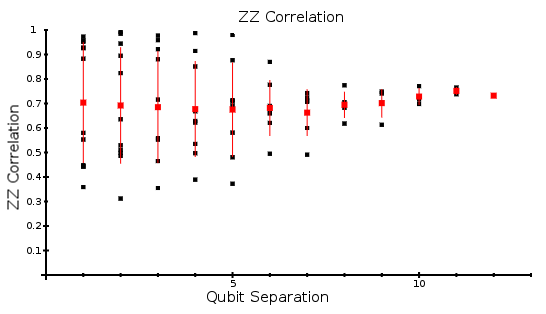
\includegraphics[width=0.9\textwidth]{images_caltech/corrdecay.png}
\captionof{figure}{\label{fig:corrdecay} ZZ\nicole{-}correlation\nicole{--}length\nicole{--}decay analysis of the final state shown in Figure~\ref{fig:colorful}: $\langle Z_i Z_j \rangle$ is plotted against $|i - j|$ for all pairs of qubits. Instead of \sout{observing a decay} \nicole{decaying}, \nicole{the} correlation remains constant as a function of distance.}
\end{Figure}


\section*{Conclusion\nicole{s}}

Quantum many-body systems have diverse and interesting properties that are often \sout{counter-intuitive} \nicole{counterintuitive.} 
\nicole{[Maybe, instead of emphasizing just how QCAs differ from expectations (based on real physical systems), emphasize that QCAs partially reflect real systems' behaviors and are partially counterintuitive? If we present QCAs just as counterintuitive in the conclusions, physicists might infer that QCAs are unrealistic and therefore worth considering only insofar as QCAs are fun games. Some physicists read only papers' abstracts, introductions, and conclusions. So what we emphasize in the conclusions matters. :)]}
Understanding these systems is essential for condensed\nicole{-}matter physics. While perspectives \nicole{tools?} like area laws and correlation-length decay have been developed for their study, concrete examples are key to understanding their behavior in a variety of situations. 
\nicole{[I'm not sure whom you refer to with ``their.'' Condensed-matter systems or QCAs?]}
This is also true for ideas in quantum information science, including entanglement monotones like negativity and concurrence. \nicole{[Again, I'm not certain whether these functions are technically monotones. Maybe you are, though.]}

Cellular automata \hl{serve as complexity generators} \nicole{generate complexity?} in classical studies. By generalizing block cellular automata \sout{using} \nicole{with} quantum circuits\nicole{,} they can also generate quantum complexity.
Using a matrix product state simulation, examples of states with interesting entanglement structure can be generated efficiently. Therefore when developing \sout{new} ideas \nicole{tools?} to \sout{help} understand many-body entanglement, or \nicole{when} building intuition \sout{on} \nicole{about} existing \sout{ones} \nicole{[More precise word recommended]}, quantum cellular automata are a helpful tool.

\nicole{[It sounds a little like you ran out of steam by the time you arrived at the conclusion. :) But the paper itself contains strong examples and justifications! The paper deserves a strong ending. Might we sharpen the conclusions?]}

\section*{Acknowledgments}

\nicole{[I recommend thanking Jenia.]}

This project would not have been possible without guidance and advice from many people. I would like to thank:

\begin{itemize}
    \item my advisers Nicole Yunger Halpern and Ning Bao for continued support throughout the project, guidance with weekly meetings and feedback on my results and writing,
    \item John Preskill for giving me the opportunity to work in an advanced research group, as well as comments on project directions and useful questions,
    \item Lincoln Carr, David Vargas and Logan Hillberry at the Colorado School of Mines, as well as Simone Montenegro at the Institute for Quantum Information in Ulm, for a great collaboration and continued insights about different approaches.

\end{itemize}

\begin{thebibliography}{5}
    \bibitem{Bleh} D. Bleh, T. Calarco, S. Montangero ``Quantum Game of Life'', http://arxiv.org/abs/1010.4666, 2012
    \bibitem{Margolus} N. Margolus, ``Crystalline Computation'', Chapter 18 of \textit{Feynman and Computation} (\textsc{A. Hey}, ed.), Perseus Books (1999)
    \bibitem{Orus} R. Orus. ``A Practical Introduction to Tensor Networks: Matrix Product States and Projected Entangled Pair States''
    \bibitem{Verstraete} F. Verstraete, J.I. Cirac, V. Murg ``Matrix Product States, Projected Entangled Pair States, and variational renormalization group methods for quantum spin systems'' \mbox{arXiv:0907.2796v1}
    \bibitem{Raussendorf} R. Raussendorf, ``Quantum cellular automaton for universal quantum computation'' \mbox{10.1103/PhysRevA.72.022301}
    \bibitem{Carr} D Vargas, L. Carr ``Detecting Quantum Phase Transitions via Mutual Information Complex Networks'' \mbox{arXiv:cond-mat.stat-mech/1508.07041}
    \bibitem{Brennen} G. K. Brennen, J. E. Williams, ``Entanglement Dynamics in 1D Quantum Cellular Automata'' \mbox{ arXiv:quant-ph/0306056v1}
    \bibitem{Ziman} M. Ziman, P. Stelmachovic, V. Buzek, M. Hillery, V. Scarani, N. Gisin "Quantum Homogenization" \mbox{arXiv:quant-ph/0110164}
%    \bibitem{Schulman} L. S. Schulman and P. E. Seiden, ``Statistical Mechanics of a Dynamical System Based on Conway's Game of Life'', Journal of Statistical Physics, Vol. 19, No. 3, 1978
%    \bibitem{Crooks} G. Crooks, ``Entropy production fluctuation theorem and the nonequilibrium work relation for free energy differences'', http://arxiv.org/abs/cond-mat/9901352v4, 1999
%   \bibitem{Jarzynski} C. Jarzynski, ``Nonequilibrium Equality for Free Energy Differences'', Journal of Statistical Physics, Vol. 78, No. 14, 1997
\end{thebibliography}






\end{multicols}

\end{document}
